%%%%%%%%%%%%%%%%%%%%%%%%%%%%%%%%%%%%%%%%%%%%%%%%%%%%%%%%%%%%%%%%%%%%%%%%%%%%%%%%
\chapter{Αποτελέσματα}

%%%%%%%%%%%%%%%%%%%%%%%%%%%%%%%%%%%%%%%%%%%%%%%%%%%%%%%%%%%%%%%%%%%%%%%%%%%%%%%%
\section{Καταγραφή της Κίνησης}

Ως αποτελέσματα της καταγραφής της κίνησης επιλέχθηκε αρχικά να παρουσιαστεί η ικανότητα καταγραφής του μήκους των τμημάτων του ανθρώπινου σώματος. Στο πείραμα συμμετείχαν δύο δείγματα τα οποία εκτέλεσαν διαφορετικές κινήσεις, όπου για κάθε κίνηση υπολογίστηκε το μέσο μήκος των τμημάτων του σώματος. Αφού συγκεντρώθηκαν τα αποτελέσματα, κατασκευάστηκαν τα αντίστοιχα διαγράμματα που δείχνουν το μέσο μήκος από όλες τις καταγεγραμμένες κινήσεις για κάθε τμήμα μαζί με τις αντίστοιχες τυπικές αποκλίσεις.

\begin{figure}[H]
    \centering
    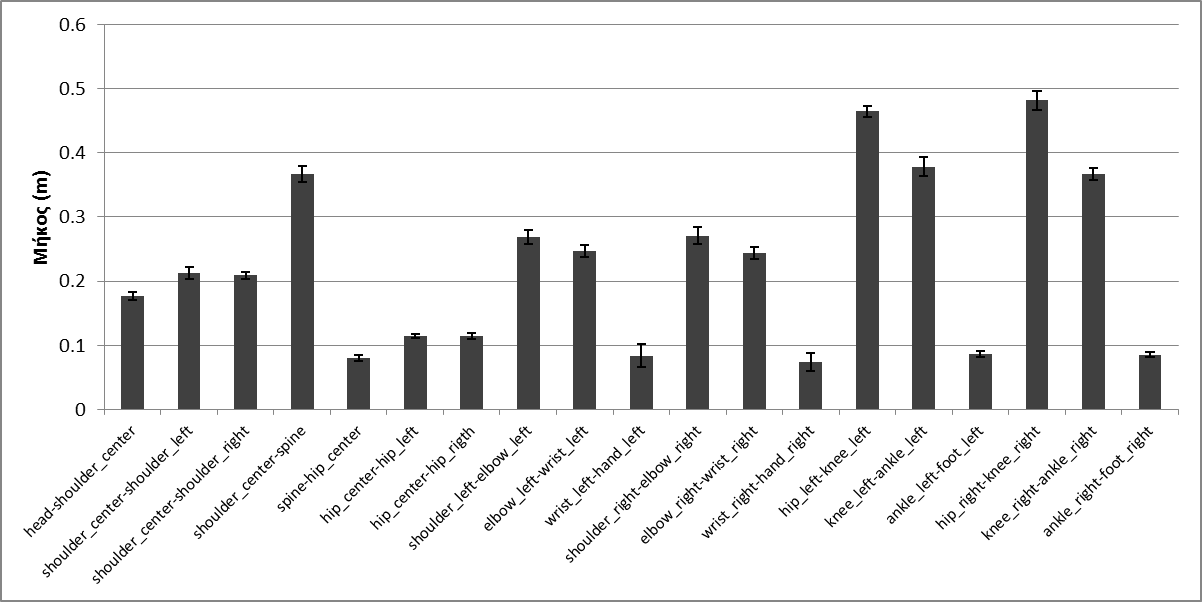
\includegraphics[width=.9\textwidth]{fig/subject01-segments.png}
    \caption{Μήκη τμημάτων για το πρώτο δείγμα (14 κινήσεις)}
    \label{fig:subject01-segments}
\end{figure}

Παρατηρούμε ότι οι τυπικές αποκλίσεις είναι μικρές με ελάχιστη για το πρώτο δείγμα στα $std_{min} = 0.0030m$ και με μέγιστη τιμή στα $std_{max} = 0.0182m$ \ref{fig:subject01-segments}. Όσον αφορά το δεύτερο δείγμα οι αντίστοιχες τυπικές αποκλίσεις είναι $std_{min} = 0.0.0019m$, $std_{max} = 0.0146m$ αντίστοιχα \ref{fig:subject02-segments}.

\begin{figure}[H]
    \centering
    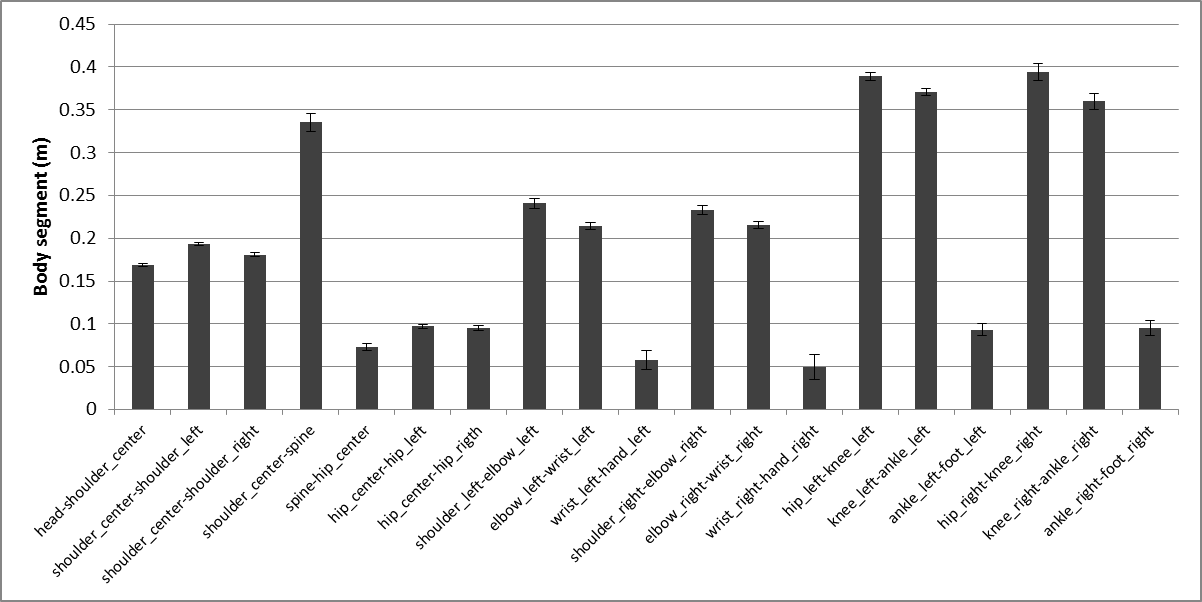
\includegraphics[width=.9\textwidth]{fig/subject02-segments.png}
    \caption{Μήκη τμημάτων για το δεύτερο δείγμα (5 κινήσεις)}
    \label{fig:subject02-segments}
\end{figure}

Ως δεύτερη σύγκριση του συστήματος, καταγράφτηκε μια κίνηση χωρίς την χρήση κάποιου φίλτρου και στην συνέχεια καταγράφτηκε όμοια κίνηση με χρήση φίλτρου και ως παράμετροι επιλέχθηκαν οι τιμές για δυνατό φιλτράρισμα από τον πίνακα \ref{tab:filter-parameters}. Επίσης έγινε μια απλή υλοποίηση ενός φίλτρου \eng{Kalman} με βάση την εξής αναδρομική σχέση \ref{equ:kalman-predict-update} και επιλέχθηκαν τιμές για τα $R = 0.05,\; Q = 0.05$. Στον πίνακα \ref{tab:no-filter-filter-kalman} στην αριστερή στήλη είναι οι συντεταγμένες του δεξιού χεριού χωρίς την χρήση κάποιου φίλτρου, ενώ στην δεξιά στήλη με χρήση του δυνατού φίλτρου. Με διακεκομμένες γραμμές φαίνεται η απόκριση του φίλτρου \eng{Kalman}. Στην περίπτωση που επιλέξουμε να χρησιμοποιήσουμε δυνατό φίλτρο δεν διακρίνεται βελτιώση αν χρησιμοποιήσουμε του φίλτρου \eng{Kalman}, όπως έχει υλοποιηθεί. Φαίνεται όμως η ανάγκη για εξομάλυνση, οπότε απλά φίλτρα που φιλτράρουν τις απότομες μεταβολές βελτιώνουν πολύ το αποτέλεσμα.

\begin{equation}
    \begin{gathered}
        \text{Πρόβλεψη} \\
        \hat{p}_{t} = p_{t-1} + u_{t}, \quad u_{t} = \frac{p_{t-1} - p_{t-2}}{t_{t-1} - t_{t-2}} \\
        \hat{P} = P_{t-1} + Q \\[.5cm]
        \text{Διόρθωση} \\
        Κ = \frac{\hat{P}}{\hat{P} + R}\\
        p_{t} = \hat{p}_{t} + K \cdot (p_{t} - \hat{p}_{t}) \\
        P_{t} = (1 - K) \cdot \hat{P}
    \end{gathered}
    \label{equ:kalman-predict-update}
\end{equation}

\begin{center}
    \begin{tabular}{cc}
        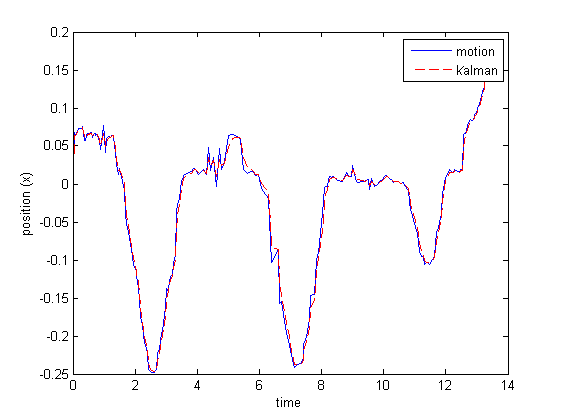
\includegraphics[width=.5\textwidth, height = 0.23\textheight, keepaspectratio]{fig/filter0-x.png} & 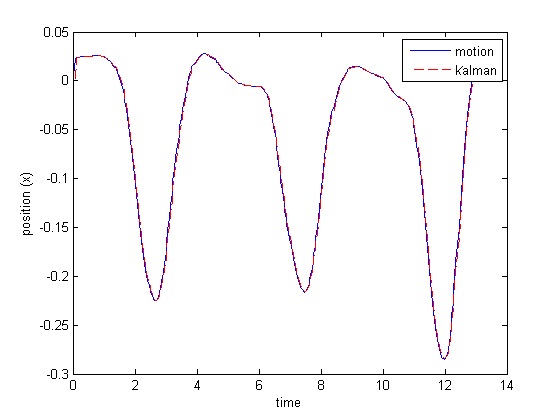
\includegraphics[width=.5\textwidth, height = 0.23\textheight, keepaspectratio]{fig/filter3-x.png}\\
        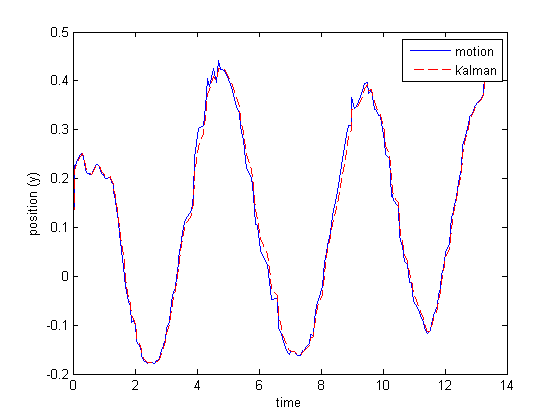
\includegraphics[width=.5\textwidth, height = 0.23\textheight, keepaspectratio]{fig/filter0-y.png} & 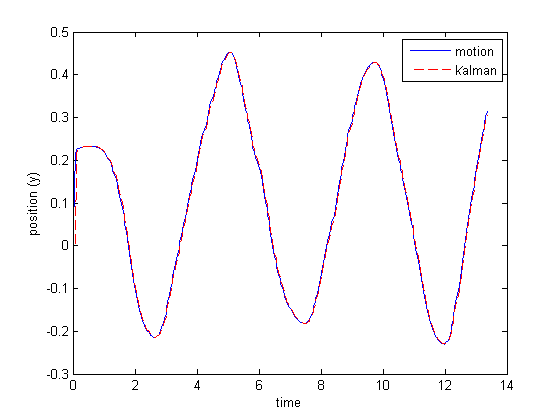
\includegraphics[width=.5\textwidth, height = 0.23\textheight, keepaspectratio]{fig/filter3-y.png}\\
        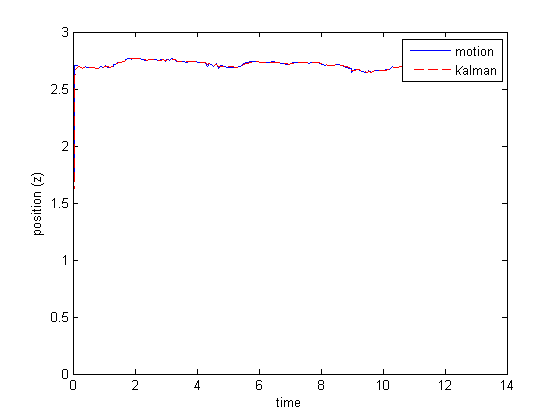
\includegraphics[width=.5\textwidth, height = 0.23\textheight, keepaspectratio]{fig/filter0-z.png} & 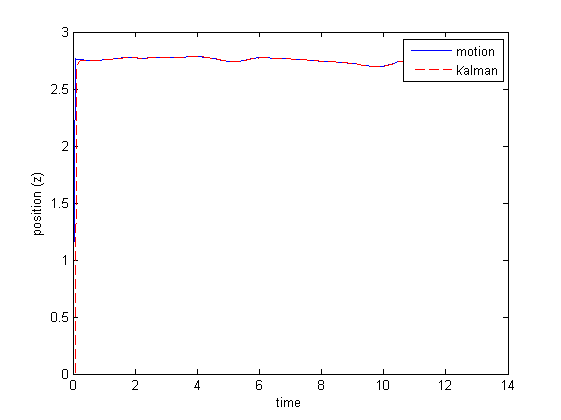
\includegraphics[width=.5\textwidth, height = 0.23\textheight, keepaspectratio]{fig/filter3-z.png}\\
        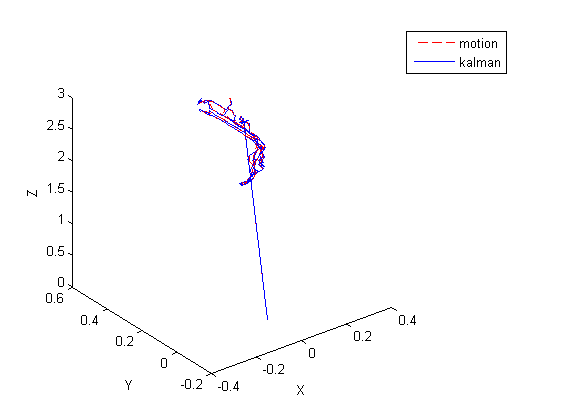
\includegraphics[width=.5\textwidth, height = 0.23\textheight, keepaspectratio]{fig/filter0-xyz.png} & 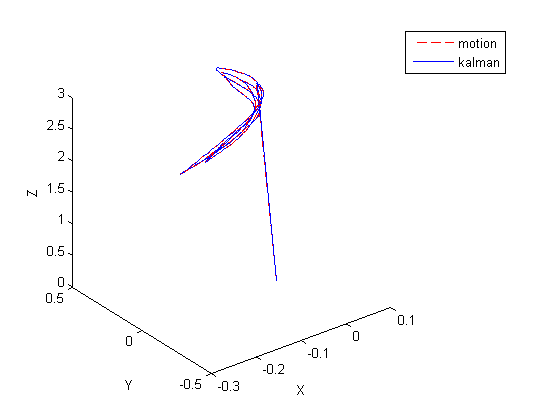
\includegraphics[width=.5\textwidth, height = 0.23\textheight, keepaspectratio]{fig/filter3-xyz.png}
    \end{tabular}
    \captionof{table}{Συντεταγμένες του δεξιού χεριού χωρίς φιλτράρισμα αριστερά και με φιλτράρισμα δεξιά}
    \label{tab:no-filter-filter-kalman}
\end{center}

%%%%%%%%%%%%%%%%%%%%%%%%%%%%%%%%%%%%%%%%%%%%%%%%%%%%%%%%%%%%%%%%%%%%%%%%%%%%%%%%
\section{Αντίστροφη Κινηματική}

Για να υπάρξουν σωστά αποτελέσματα κατά την αντίστροφη κινηματική είναι αναγκαία η διαδικασία της κανονικοποίησης, ώστε το γενικό μοντέλο να πάρει τις διαστάσεις του δείγματος. Οπότε η διαδικασία της κανονικοποίησης θεωρείται δεδομένη κάθε φορά. Αυτό που μπορούμε να εκθέσουμε ως αποτέλεσμα της διαδικασίας είναι το σφάλμα της αντίστροφης κινηματικής. Για το πείραμα εκτελέστηκε η αντίστροφη κινηματική για 6 διαφορετικές κινήσεις του ίδιου δείγματος και καταγράφηκε το συνολικό τετραγωνικό σφάλμα (\eng{total square error}), το σφάλμα λόγω ενδείξεων (\eng{marker error}) και το μέγιστο σφάλμα από όλες τις αρθρώσεις (\eng{max joint error}). Τα τρία αυτά σφάλματα ήταν διαθέσιμα για κάθε χρονική στιγμή που υπολογίζονταν η αντίστροφη κινηματική. Ως εκ τούτο για κάθε ένα από αυτά τα σφάλματα υπολογίστηκε η μέση τιμή, η τυπική απόκλιση και η μέγιστη τιμή από όλες τις χρονικές στιγμές για κάθε κίνηση ξεχωριστά.

\begin{center}
    \begin{tabular}{cc}
        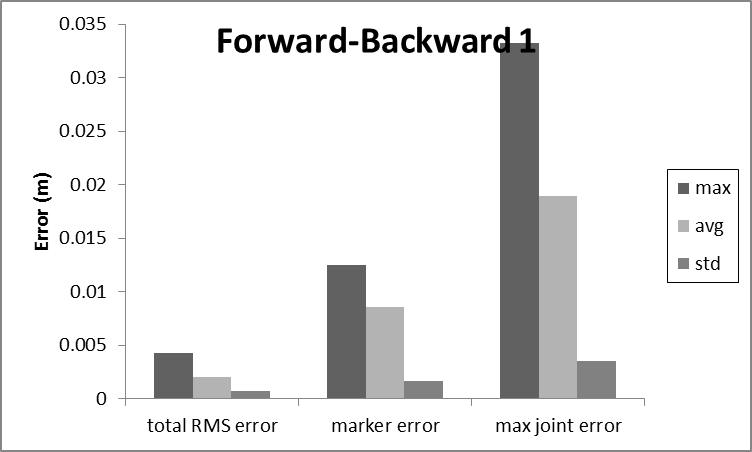
\includegraphics[width=.48\textwidth, keepaspectratio]{fig/ik-reg1.png} & 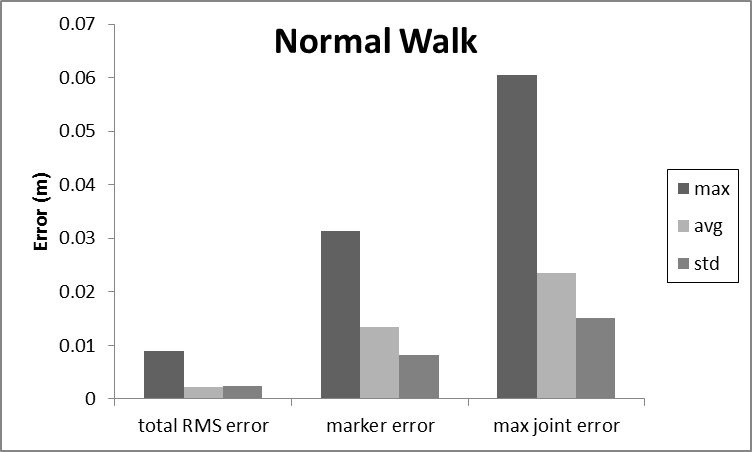
\includegraphics[width=.48\textwidth, keepaspectratio]{fig/ik-reg2.png}\\[3pt]
        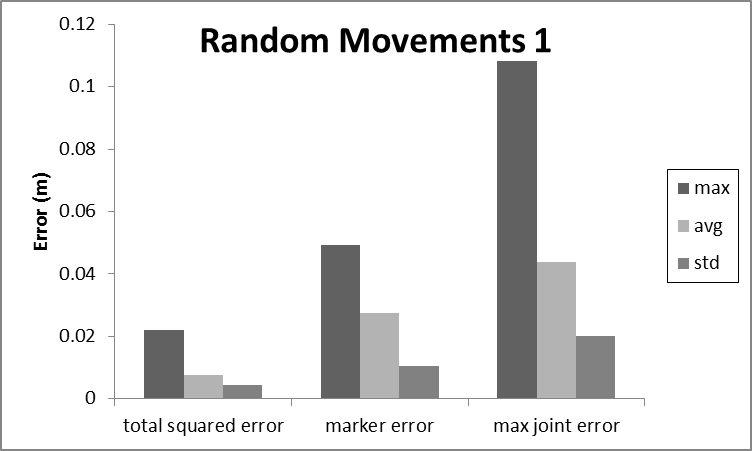
\includegraphics[width=.48\textwidth, keepaspectratio]{fig/ik-reg3.png} & 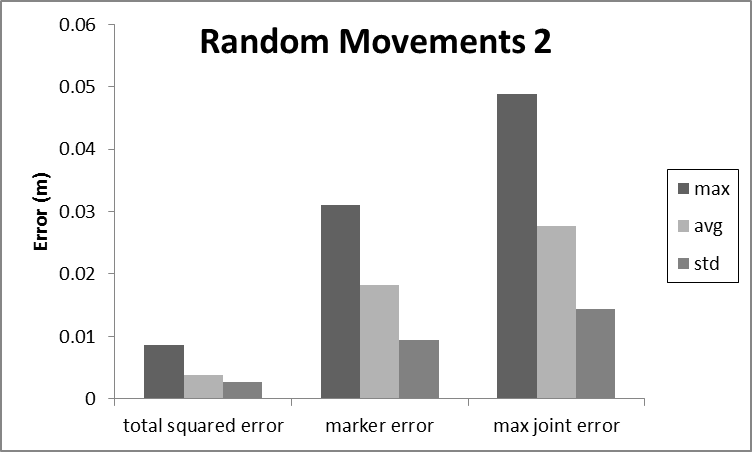
\includegraphics[width=.48\textwidth, keepaspectratio]{fig/ik-reg4.png}\\[3pt]
        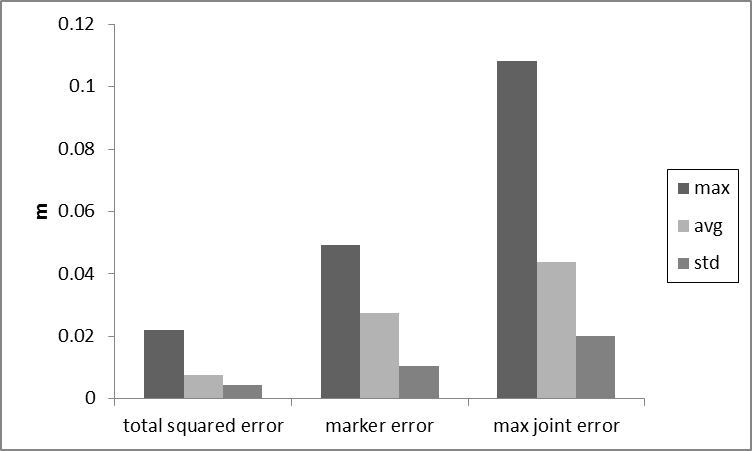
\includegraphics[width=.48\textwidth, keepaspectratio]{fig/ik-reg5.png} & 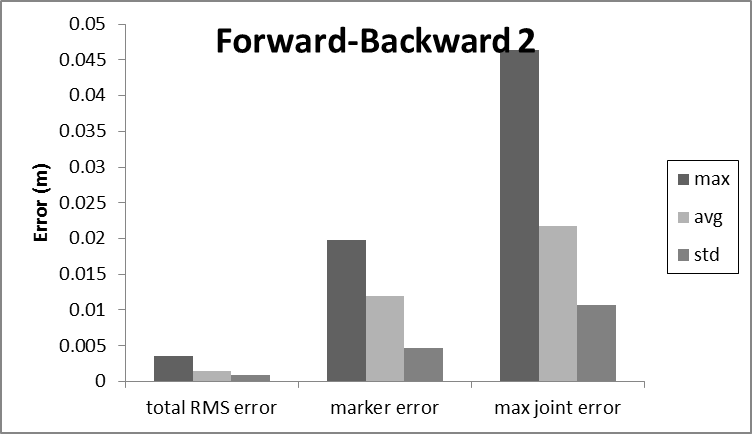
\includegraphics[width=.48\textwidth, keepaspectratio]{fig/ik-reg6.png}
    \end{tabular}
    \captionof{table}{Τα σφάλματα της αντίστροφης κινηματικής ανά κίνηση}
    \label{tab:ik-error-regions}
\end{center}

Στην εικόνα \ref{fig:ik-no-scale-with-scale} έγινε σύγκριση της αποτελεσματικότητας της διαδικασία κανονικοποίησης στο αποτέλεσμα της αντίστροφης κινηματικής. Η πρώτη τριάδα των μετρήσεων αφορά τα σφάλματα της αντίστροφης κινηματικής χωρίς την διεξαγωγή κανονικοποίησης, ενώ η δεύτερη τριάδα με διεξαγωγή της κανονικοποίησης. Παρατηρείται μεγάλη βελτίωση των σφαλμάτων και ιδιαίτερα στα σφάλματα μέσης τιμής. Ωστόσο παρατηρείται ότι δεν βελτιώνεται ιδιαίτερα το σφάλμα της μέγιστης τιμής σφάλματος της άρθρωσης. Δηλαδή υπάρχουν κάποιες αρθρώσεις που δίνουν μεγάλο σφάλμα, αλλά γενικά έχουμε βελτίωση ως προς το μέσο όρο των αρθρώσεων.

\begin{figure}[H]
    \centering
    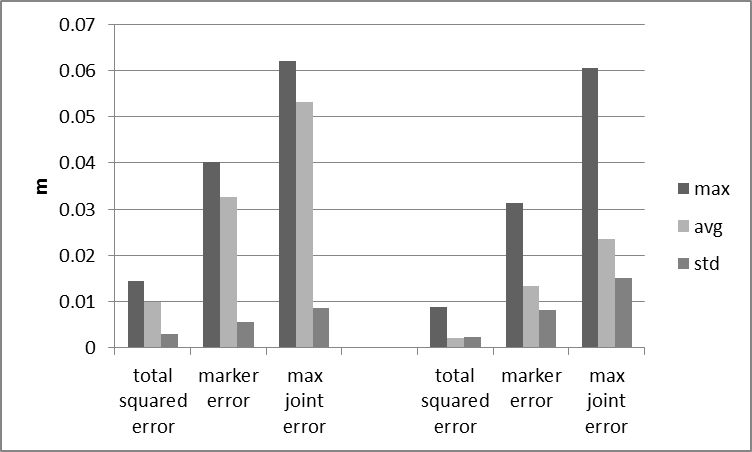
\includegraphics[width=0.8\textwidth, keepaspectratio]{fig/ik-no-scale-with-scale.png}
    \caption{Σύγκριση της αποδοτικότητας της κανονικοποίησης}
    \label{fig:ik-no-scale-with-scale}
\end{figure}

%%%%%%%%%%%%%%%%%%%%%%%%%%%%%%%%%%%%%%%%%%%%%%%%%%%%%%%%%%%%%%%%%%%%%%%%%%%%%%%%
\section{Αντίστροφη Δυναμική}

Με την αντίστροφη δυναμική έχουμε στην διάθεση μας τις ροπές που ασκούνται στις αρθρώσεις κάθε χρονική στιγμή. Λόγω της δυσκολίας υπολογισμού των εξωτερικών δυνάμεων, χρησιμοποιήθηκαν δεδομένα βάδισης και καταγεγραμμένη αντίδραση εδάφους που βρέθηκε στο διαδίκτυο, ώστε να επιβεβαιωθεί η ισχύς της ανάλυσης. Στην μελέτη των δυνάμεων, παρουσιάζονται οι ροπές του γοφού, του γονάτου και του αστράγαλου σε ένα κύκλο βάδισης και συγκρίνονται με την βιβλιογραφία \cite{whittlesey}. Στον πίνακα \ref{tab:id-hip-knee-ankle-moments} από αριστερά είναι οι πειραματικές ροπές για έναν κύκλο βάδισης και από δεξιά είναι τα αντίστοιχα με βάση της βιβλιογραφίας. Τα δικά μας διαγράμματα είναι ανάποδα γιατί έχουμε θεωρήσει διαφορετικές φορές στους βαθμούς ελευθερίας, ωστόσο τα αποτελέσματα μας συμβαδίζουν με εκείνα της βιβλιογραφίας αν λάβουμε υπόψιν τις ενδείξεις πάνω στα διαγράμματα.

\begin{center}
    \begin{tabular}{cc}
        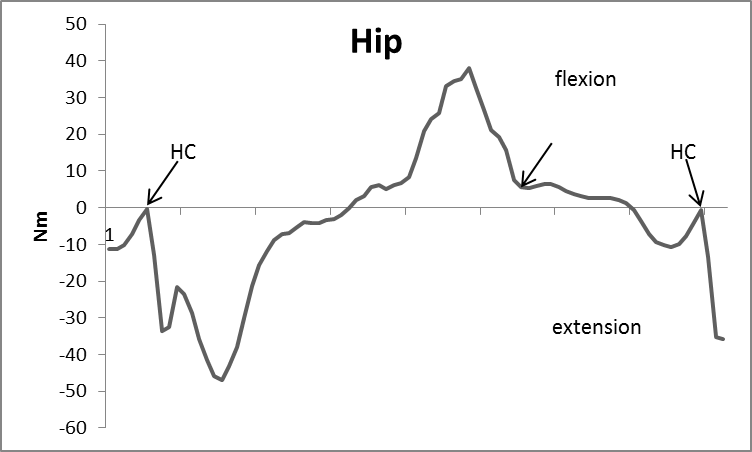
\includegraphics[width=.48\textwidth, keepaspectratio]{fig/id-hip.png} & 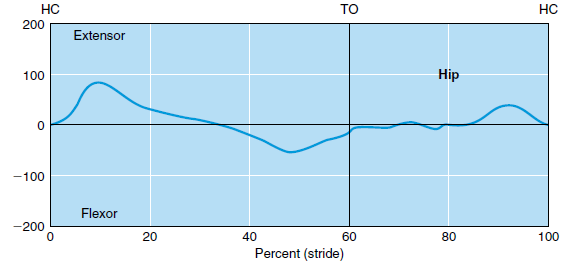
\includegraphics[width=.48\textwidth, keepaspectratio]{fig/id-hip-ref.png}\\[3pt]
        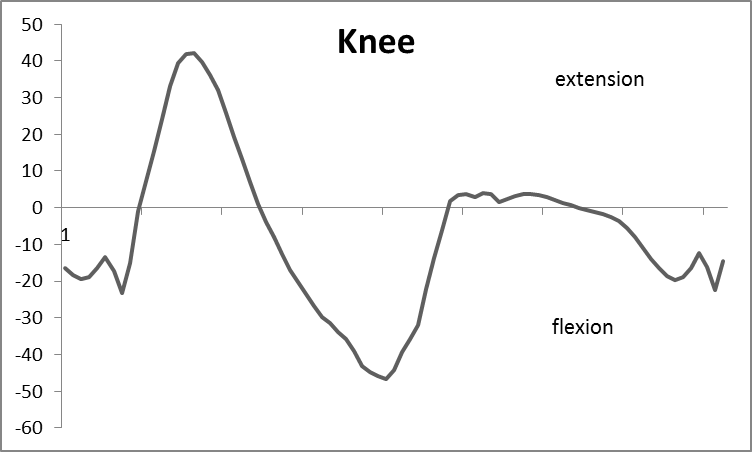
\includegraphics[width=.48\textwidth, keepaspectratio]{fig/id-knee.png} & 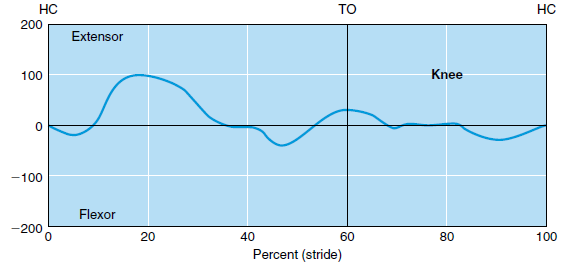
\includegraphics[width=.48\textwidth, keepaspectratio]{fig/id-knee-ref.png}\\[3pt]
        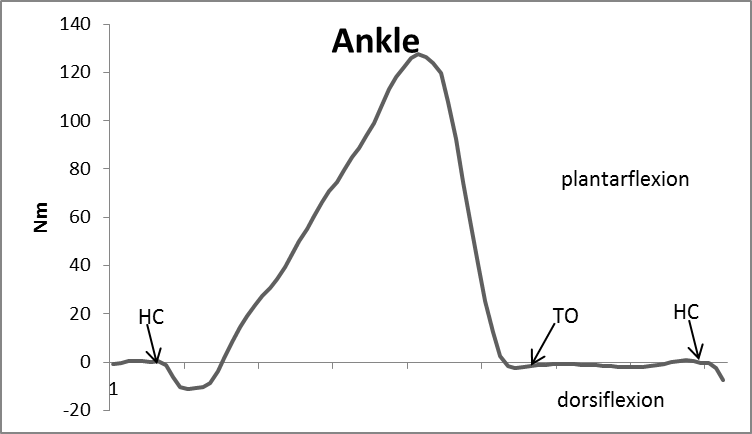
\includegraphics[width=.48\textwidth, keepaspectratio]{fig/id-ankle.png} & 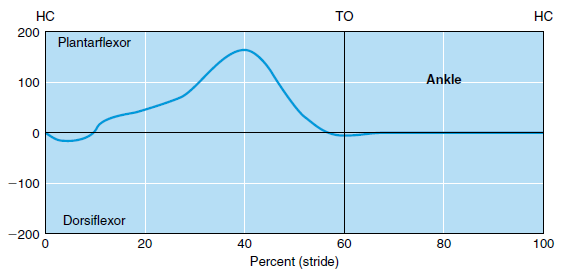
\includegraphics[width=.48\textwidth, keepaspectratio]{fig/id-ankle-ref.png}
    \end{tabular}
    \captionof{table}{Σύγκριση ροπών για ένα κύκλο βάδισης}
    \label{tab:id-hip-knee-ankle-moments}
\end{center}

%%%%%%%%%%%%%%%%%%%%%%%%%%%%%%%%%%%%%%%%%%%%%%%%%%%%%%%%%%%%%%%%%%%%%%%%%%%%%%%%
\section{Μυϊκή Συσχέτιση}

Στο παρακάτω σχήμα \ref{fig:iber-length-vs-knee-angle} φαίνεται πώς μπορούμε μέσα από την γεωμετρική τοποθέτηση των μυών να εκτιμήσουμε το μήκος τους και πως αυτό μεταβάλλεται με την αλλαγή της γωνίας της άρθρωσης δράσεως. Οι δύο μύες ο \eng{rectus femoris} και \eng{vastus intermedius} δρουν στο γόνατο ως καμπτήρες. Ο \eng{rectus femoris} είναι ένας μυς που ξεκινά από την λεκάνη και καταλήγει στην επιγονατίδα, ενώ  ο \eng{vastus intermedius} ξεκινά από την μέση του μηρού και καταλήγει πάλι στην επιγονατίδα. Είναι προφανές ότι όταν το πόδι είναι τεντωμένο τα μήκη των δύο μυών είναι ελάχιστα, ενώ όταν το γόνατο λυγίζει τότε μεγαλώνει το μήκος τους.

\begin{figure}[H]
    \centering
    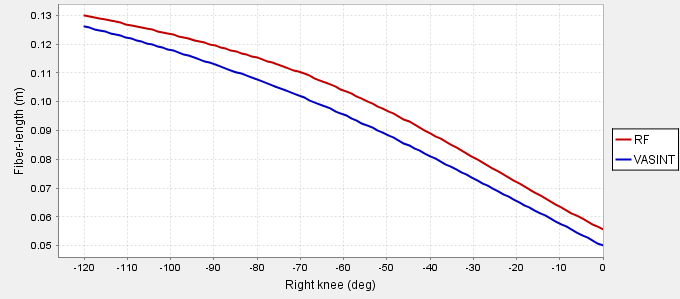
\includegraphics[width=0.8\linewidth, keepaspectratio]{fig/fiber-length-vs-knee-angle.png}
    \caption{Μίκη μυών συνάρτηση της γωνίας της άρθρωσης του γονάτου}
    \label{fig:iber-length-vs-knee-angle}
\end{figure}

Στο δεύτερο διάγραμμα \ref{fig:moment-arm-vs-knee-angle} γίνεται μια γεωμετρική ερμηνεία που σχετίζεται με την τοποθέτηση των μυών. Η παράμετρος είναι η ποσότητα που μετατρέπει την δύναμη που παράγει ο μυς σε ροπή στην άρθρωση, η λεγόμενη ροπή αδράνειας του μυ (\eng{muscle moment arm}). Το σημείο ασυνέχειας (-85 μοίρες) που παρατηρείται, οφείλεται στο γεγονός ότι για την συγκεκριμένη γωνία οι μύες ξεκινούν να τυλίγονται γύρω από την επιγονατίδα και το μήκος τους διαμερίζεται κατάλληλα με αποτέλεσμα να υπάρχουν ασυνέχειες στους υπολογισμούς.

\begin{figure}[H]
    \centering
    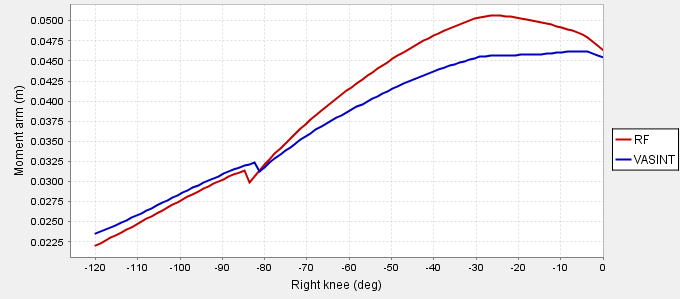
\includegraphics[width=0.8\linewidth, keepaspectratio]{fig/moment-arm-vs-knee-angle.png}
    \caption{Μίκη μυών συνάρτηση της γωνίας της άρθρωσης του γονάτου}
    \label{fig:moment-arm-vs-knee-angle}
\end{figure}

%%%%%%%%%%%%%%%%%%%%%%%%%%%%%%%%%%%%%%%%%%%%%%%%%%%%%%%%%%%%%%%%%%%%%%%%%%%%%%%%
\section{Εκτέλεση Ορθής Δυναμικής}

Σε αυτή την παράγραφο απλά θα δείξουμε την βελτίωση της ευστάθειας που πετυχαίνουμε ανάλογα με το ποια κατηγορία μεθόδων θα χρησιμοποιήσουμε. Η ευστάθεια συμβολίζει την συσσώρευση σφαλμάτων στα στάδια μέχρι τον υπολογισμό των των διεγέρσεων, που μπορεί να είναι είτε ροπές, είτε νευρικές διεγέρσεις. Στο πρώτο πείραμα μετά την αντίστροφη κινηματική εκτελούμε αντίστροφη δυναμική και τροφοδοτήσαμε στην συνέχεια τις υπολογισμένες ροπές στην διαδικασία της ορθής δυναμικής ώστε να γίνει σύγκριση. Στο δεύτερο πείραμα μετά την αντίστροφη κινηματική εκτελούμε την διαδικασία του υπολογισμού των μυϊκών διεγέρσεων όπου υπολογίζουμε τις διεγέρσεις των μυών που απαιτούνται για την παραγωγή της καταγεγραμμένης κίνησης και κατόπιν εκτελούμε ορθή δυναμική για να συγκρίνουμε το αποτέλεσμα της μεθόδου με αυτό της αντίστροφης δυναμικής. Στον πίνακα \ref{tab:fd-cmc-id} στην αριστερή στήλη είναι το ευσταθές αποτέλεσμα της μεθόδου του υπολογισμού των μυϊκών διεγέρσεων και στην δεξιά στήλη είναι το ασταθές αποτέλεσμα της αντίστροφης δυναμικής. Εξετάζονται οι γενικευμένες συντεταγμένες για τον γοφό, το γόνατο και τον αστράγαλο αντίστοιχα. Με κόκκινο είναι η επιθυμητή τροχεία που θέλουμε να πετύχουμε με βάση το αποτέλεσμα της αντίστροφης κινηματικής ενώ με μπλε το αποτέλεσμα των αναλύσεων. Παρατηρούμε την μεγάλη σύγκληση που επιτυγχάνουμε με χρήση της μεθόδου υπολογισμού των μυϊκών διεγέρσεων σε σχέση με την αντίστροφη δυναμική, ωστόσο μετά από κάποια χρονική στιγμή η προτεινόμενη μέθοδος μπαίνει και αυτή στην αστάθεια που είναι και αναμενόμενο.

\begin{center}
    \begin{tabular}{cc}
        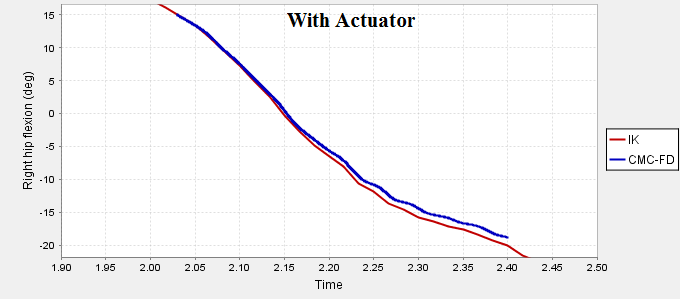
\includegraphics[width=.48\textwidth, keepaspectratio]{fig/hip-ik-cmc.png} & 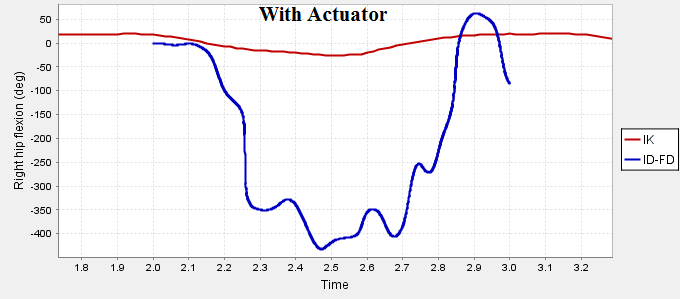
\includegraphics[width=.48\textwidth, keepaspectratio]{fig/hip-ik-id.png}\\[3pt]
        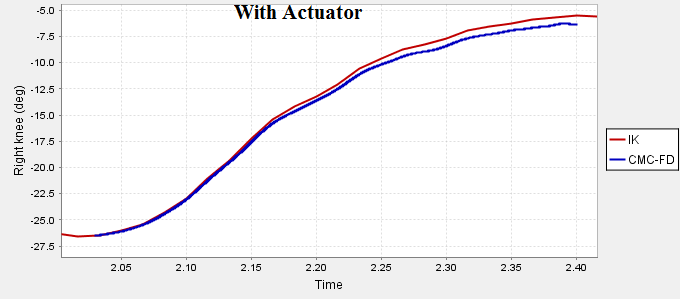
\includegraphics[width=.48\textwidth, keepaspectratio]{fig/knee-ik-cmc.png} & 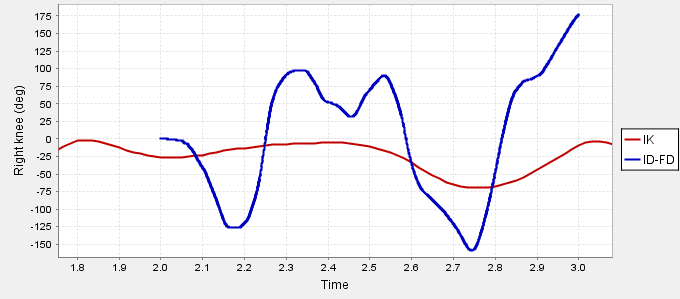
\includegraphics[width=.48\textwidth, keepaspectratio]{fig/knee-ik-id.png}\\[3pt]
        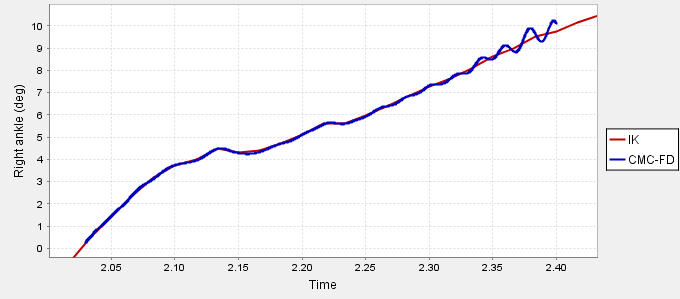
\includegraphics[width=.48\textwidth, keepaspectratio]{fig/ankle-ik-cmc.png} & 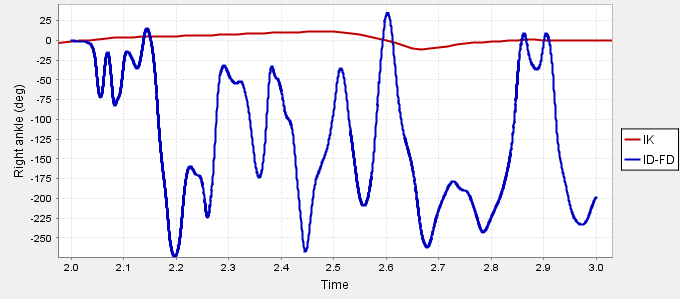
\includegraphics[width=.48\textwidth, keepaspectratio]{fig/ankle-ik-id.png}
    \end{tabular}
    \captionof{table}{Σύγκριση της ευστάθειας της ορθής δυναμικής}
    \label{tab:fd-cmc-id}
\end{center}

Στο σχήμα \ref{fig:rf-vasint-activation} αναφέρεται το αποτέλεσμα των νευρικών διεγέρσεων για του δυο μύες \eng{rectus femoris} και \eng{vastus intermedius}. Η επιβεβαίωση μπορεί να γίνει ποιοτικά με μετρήσεις από τα \eng{EMG}, ωστόσο δεν έχουμε στην διάθεση μας τέτοιες μετρήσεις, απλά αναδεικνύεται ότι μπορούμε να έχουμε αποτελέσματα ακόμη και σε νευρικό επίπεδο.

\begin{figure}[H]
    \centering
    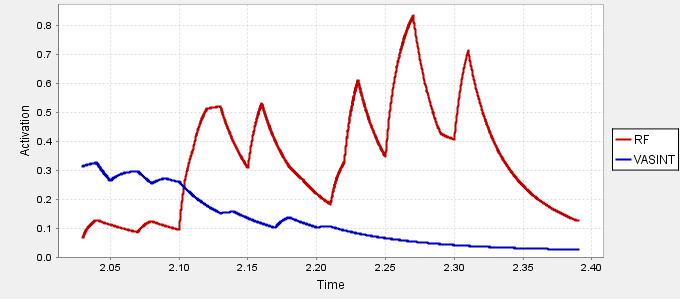
\includegraphics[width=0.8\linewidth, keepaspectratio]{fig/rf-vasint-activation.png}
    \caption{Μυϊκή ενεργοποίηση για τους δυο μύες}
    \label{fig:rf-vasint-activation}
\end{figure}

%\vfill

%%%%%%%%%%%%%%%%%%%%%%%%%%%%%%%%%%%%%%%%%%%%%%%%%%%%%%%%%%%%%%%%%%%%%%%%%%%%%%%%
\section{Συμπεράσματα}

Στην παρούσα εργασία δείξαμε ότι μπορούμε να καταγράψουμε την κίνηση του ανθρώπου με μια φτηνή συσκευή (συγκριτικά με άλλα συστήματα καταγραφής) όπως είναι το \eng{Kinect} και να πετύχουμε αξιόλογα αποτελέσματα με ελάχιστο κόπο από την μεριά του προγραμματιστή. Επιπλέον δείξαμε πως με απλές μεθόδους φιλτραρίσματος μπορεί να βελτιωθεί κατά πολύ το αποτέλεσμα της καταγεγραμμένης κίνησης, ώστε να είναι κατάλληλο για επεξεργασία στα μετέπειτα στάδια. Επίσης παρουσιάσαμε ότι το \eng{Kinect} είναι σε θέση να προσδιορίζει τα μορφομετρικά χαρακτηριστικά του ανθρώπου με μεγάλη ακρίβεια. Ωστόσο δεν καταφέραμε να ξεπεράσουμε το πρόβλημα της παρεμπόδισης (\eng{occlusion}), που όμως λύνεται αν χρησιμοποιηθούν στην καταγραφή της κίνησης παραπάνω από μια συσκευές με διαφορετική οπτική γωνία ως προς το δείγμα.

Στην συνέχεια αποδείξαμε ότι μαζί με την καταγεγραμμένη κίνηση και ένα αξιόπιστο μοντέλο μπορούν να γίνουν πολλές και διάφορες αναλύσεις, που είναι σε θέση να βοηθήσουν τους αναλυτές να εξάγουν συμπεράσματα για το δείγμα. Ως εκ τούτου, απαραίτητο στάδιο της ανάλυσης είναι η αντίστροφη κινηματική και η μείωση των σφαλμάτων είναι κομβικό σημείο στην ανάλυση. Τονίσαμε την σημασία της αντίστροφης δυναμικής ως εργαλείο ανάλυσης και παρουσιάσαμε τα αποτελέσματα της βάδισης τα οποία συμφωνούν με τη βιβλιογραφία. Παρουσιάσαμε τα αποτέλεσμα της μεθοδολογίας παραγωγής μεγαλύτερης διάρκειας ευσταθούς βάδισης που συμβάδιζαν με μικρή απόκλιση από την επιθυμητή κίνηση. Στα πλαίσια των αναλύσεων μπορούν να εξαχθούν και άλλα αποτελέσματα, όπως είναι οι νευρικές διεγέρσεις, οι δυνάμεις που ασκούν οι μύες, τα μήκη τους κατά την βάδιση και δυνάμεις αντίδρασης μεταξύ των οστών, ωστόσο η πειραματική τους επιβεβαίωση είναι δύσκολη στην πράξη.

Κατά την διάρκεια της περιγραφής των μεθόδων ανάλυσης έγιναν συγκρίσεις και αναφέρθηκαν τα μειονεκτήματα και τα πλεονεκτήματα τους. Κατά την σχεδίαση του μοντέλου έγιναν κάποιες παραδοχές που αφορούσαν την κινητικότητα του, την γεωμετρία των μυών και την κατανομή της μάζας. Όλα αυτά οδηγούν σε σφάλματα στις εκτιμώμενες ποσότητες και ανάλογα με τις ανοχές που έχουμε θέσει με βάση του προβλήματος ίσως απαιτείται εναλλακτική προσέγγιση. Ωστόσο οι προσεγγίσεις που κάναμε οδηγούν σε ορθά αποτελέσματα με μικρές αποκλίσεις από την πραγματικότητα.

Υπάρχει πολύ περιθώριο βελτίωσης η εφεύρεση νέων, πιο γρήγορων, πιο ακριβών μεθόδων. Ειδικά το θέμα του χρόνου που απαιτούν κάποιες αναλύσεις είναι καταχρηστικό πολλές φορές, αλλά και αναπόφευκτο για ένα τόσο δύσκολο πρόβλημα. Η πρόοδος των μεθόδων προσομοίωσης σε συνδυασμό με συστήματα καταγραφής και μεθόδων ανάλυσης μπορούν να χρησιμοποιηθούν στην ιατρική και σε άλλους κλάδους και να είναι δεδομένα εργαλεία στην καθημερινότητα, βελτιώνοντας την ποιότητα των υπηρεσιών.
